\newpage
\section{GUI-Prototypen}
Im Grunde besteht das Projekt aus zwei grundlegenden Prototypen. Der Loginseite und der Templateseite f"ur alle weiteren Seiten. 
Die Templateseite unterscheidet sich minimal bei den unterschiedlichen Akteuren durch ihre Funktionalit"at.

\subsection{Loginseite}
 \begin{figure}[ht!]
  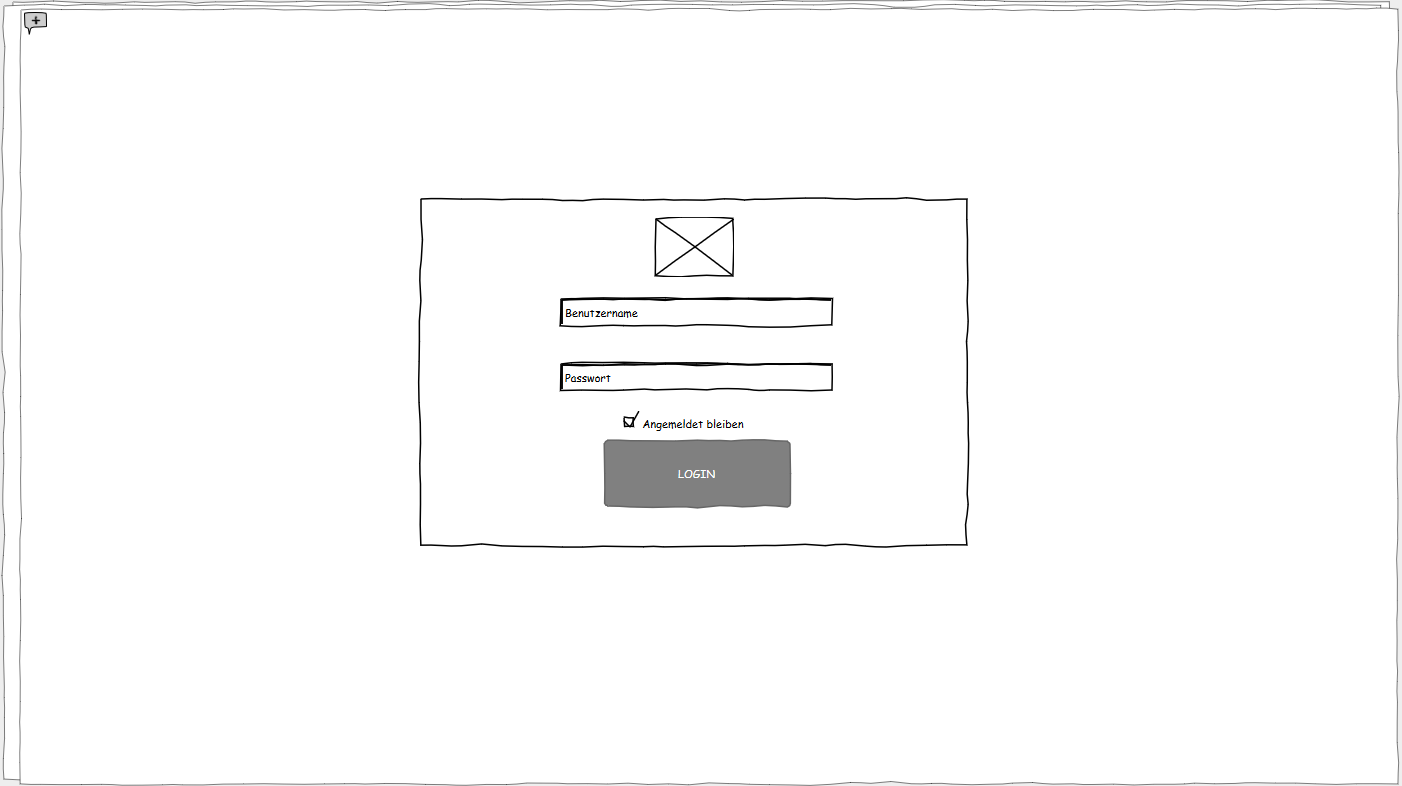
\includegraphics[width = 150mm]{pictures/Login.PNG}
 \end{figure}
 
 \newpage
 \subsection{Templateseite Elternteil}
 \begin{figure}[ht!]
  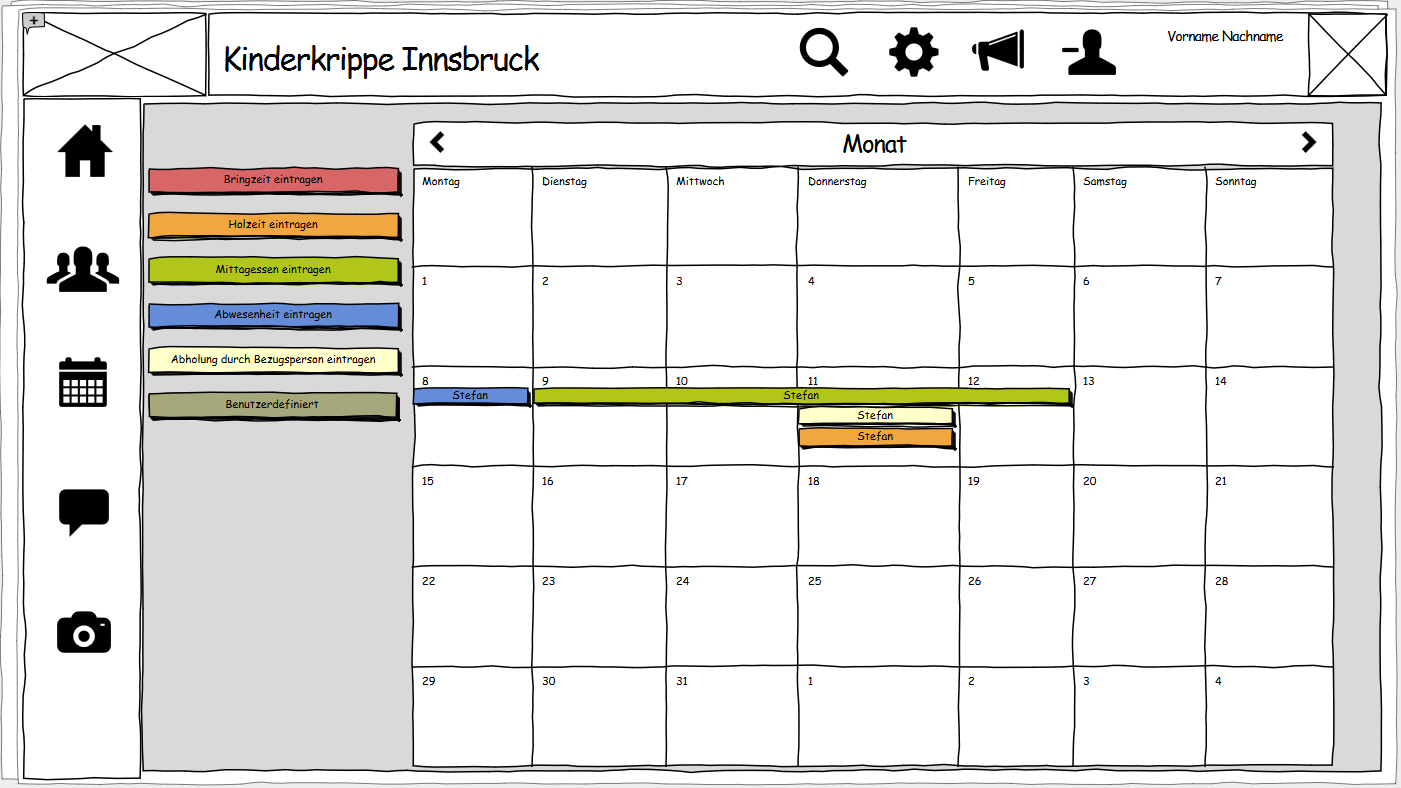
\includegraphics[width = 150mm]{pictures/Grundstellung_Elternteil.PNG}
 \end{figure}
 
  \subsection{Templateseite Mitarbeiter}
 \begin{figure}[ht!]
  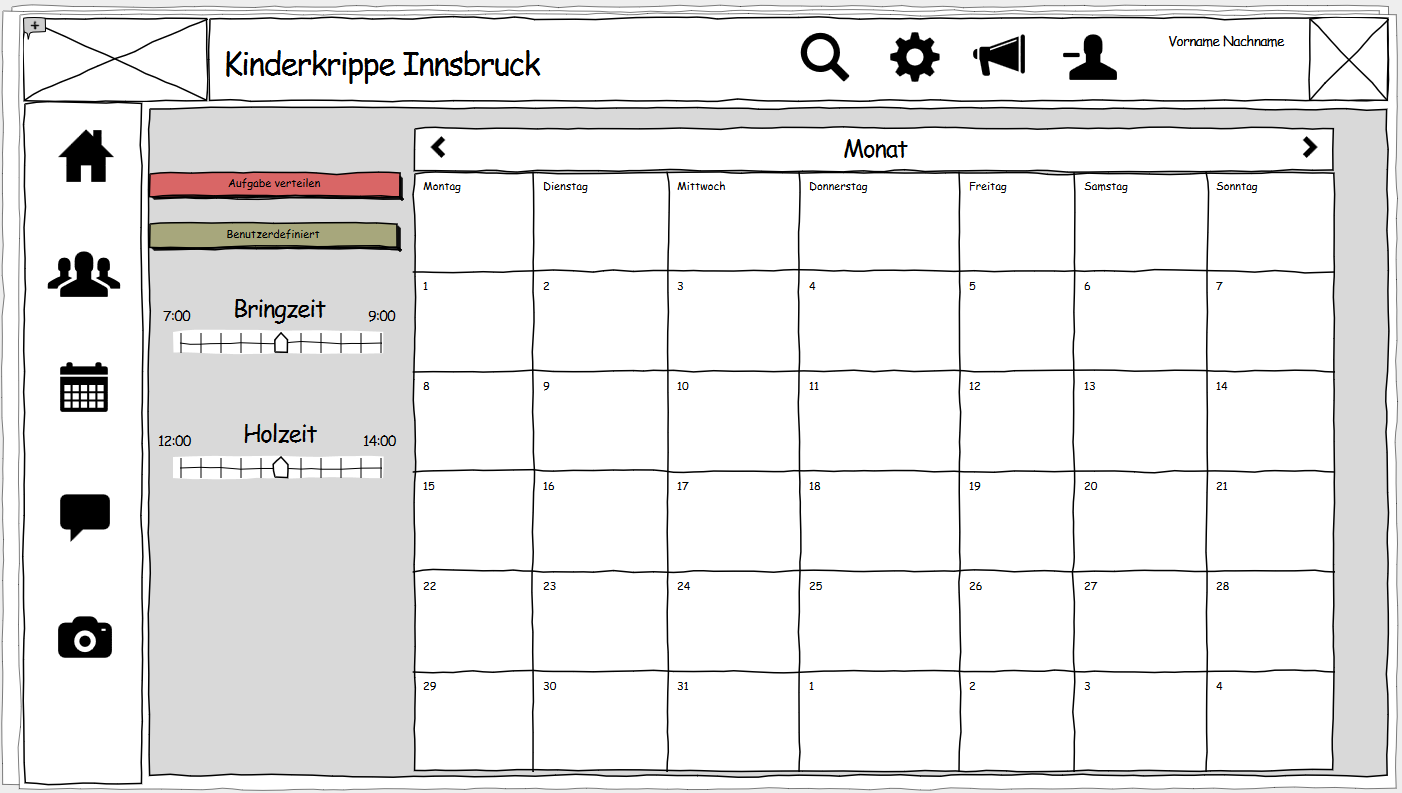
\includegraphics[width = 150mm]{pictures/Grundstellung_Mitarbeiter.PNG}
 \end{figure}
 
  \newpage
 \subsection{Templateseite Kontaktliste}
 \begin{figure}[ht!]
  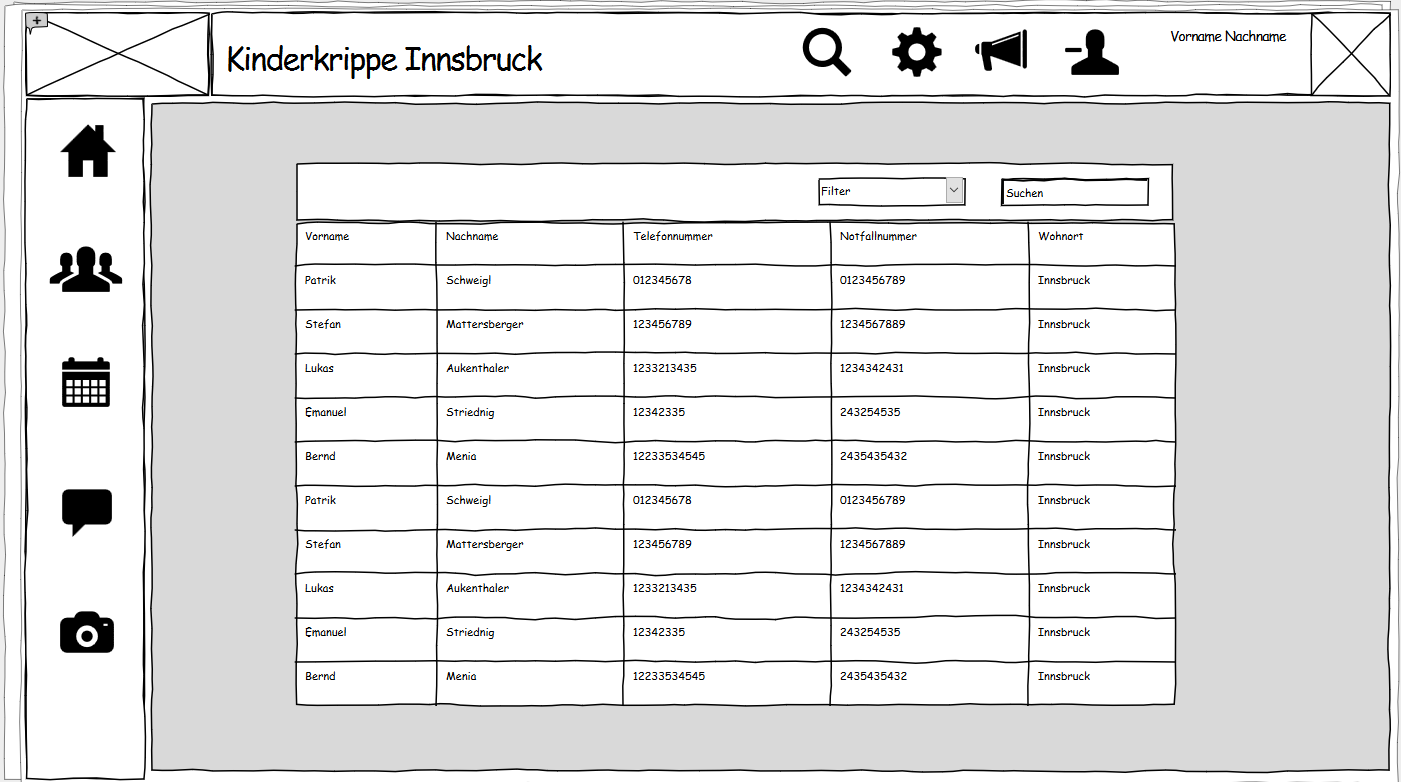
\includegraphics[width = 150mm]{pictures/Kontaktliste.PNG}
 \end{figure}
 
  \subsection{Templateseite Daten bearbeiten}
 \begin{figure}[ht!]
  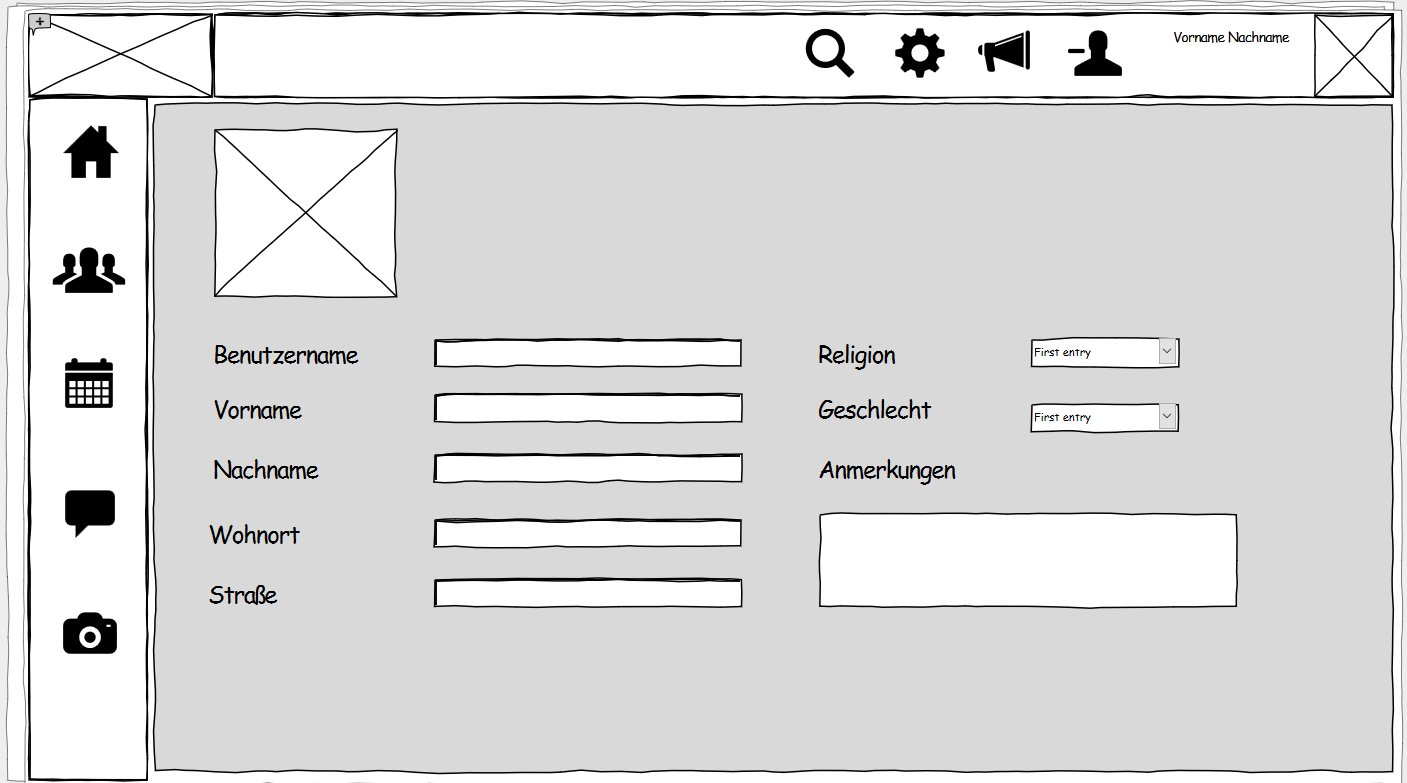
\includegraphics[width = 150mm]{pictures/daten_bearbeiten.PNG}
 \end{figure}
 
  \newpage
 \subsection{Templateseite Stammblatt}
 \begin{figure}[ht!]
  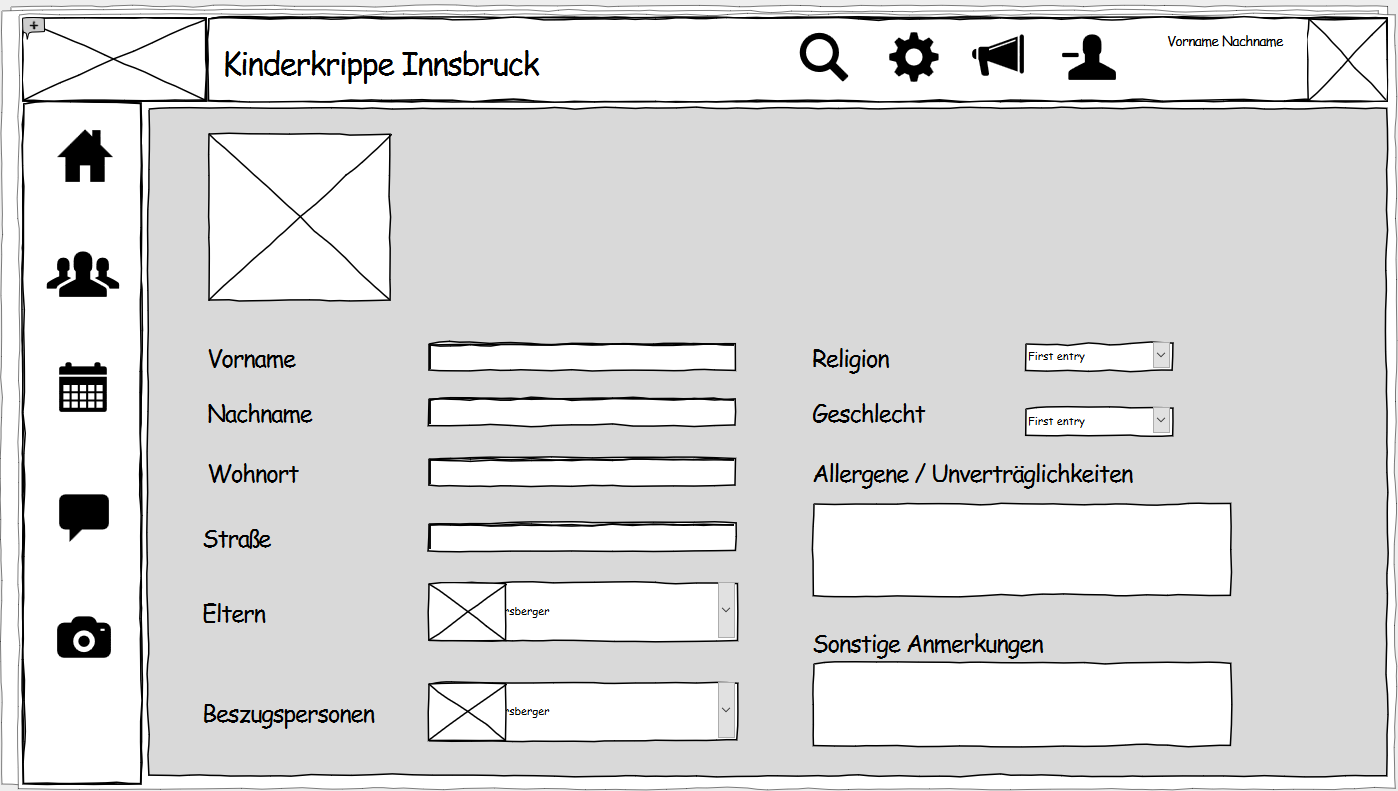
\includegraphics[width = 150mm]{pictures/Stammblattseite.PNG}
 \end{figure}
 
  \subsection{Templateseite Tagesplaner}
 \begin{figure}[ht!]
  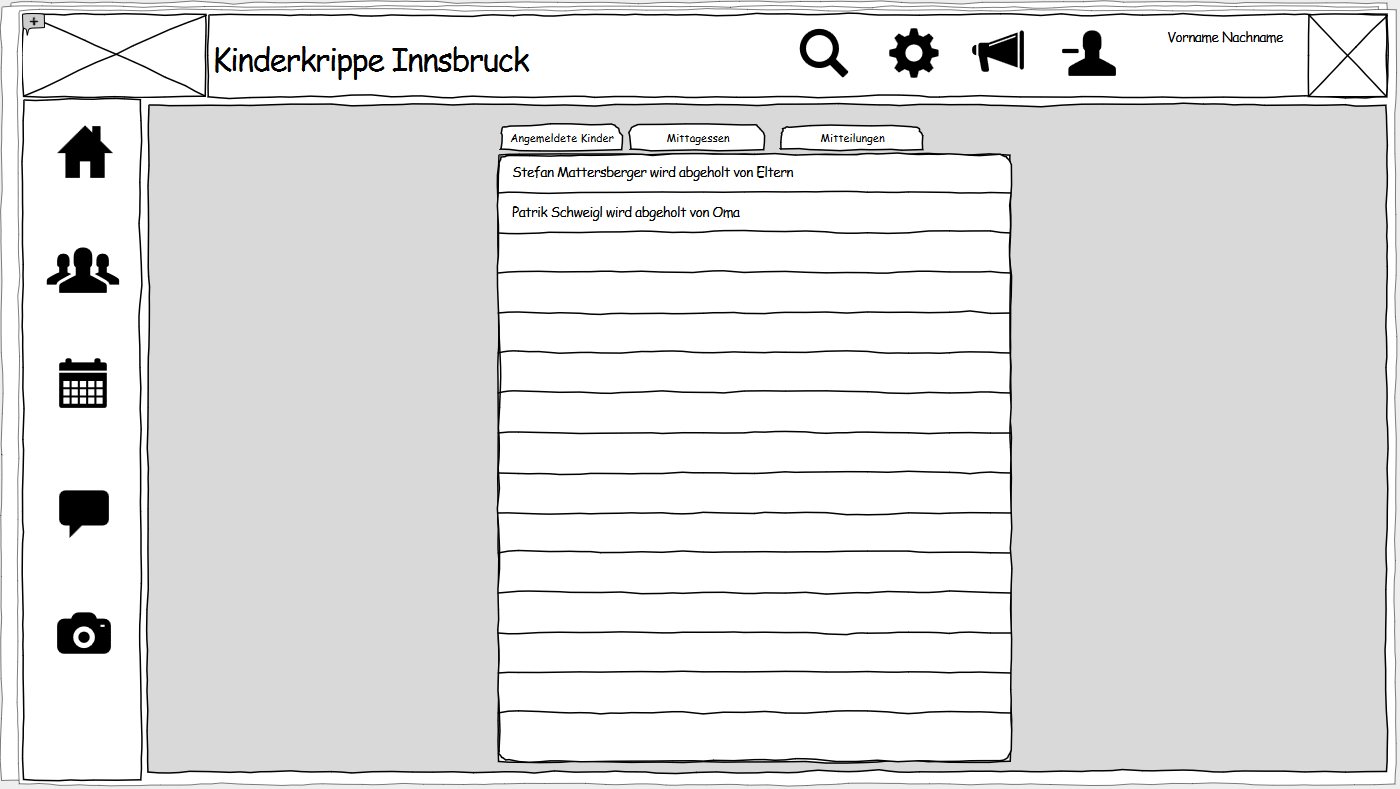
\includegraphics[width = 150mm]{pictures/Tagesplaner.PNG}
 \end{figure}
 
  \newpage
 \subsection{Templateseite Messageboard}
 \begin{figure}[ht!]
  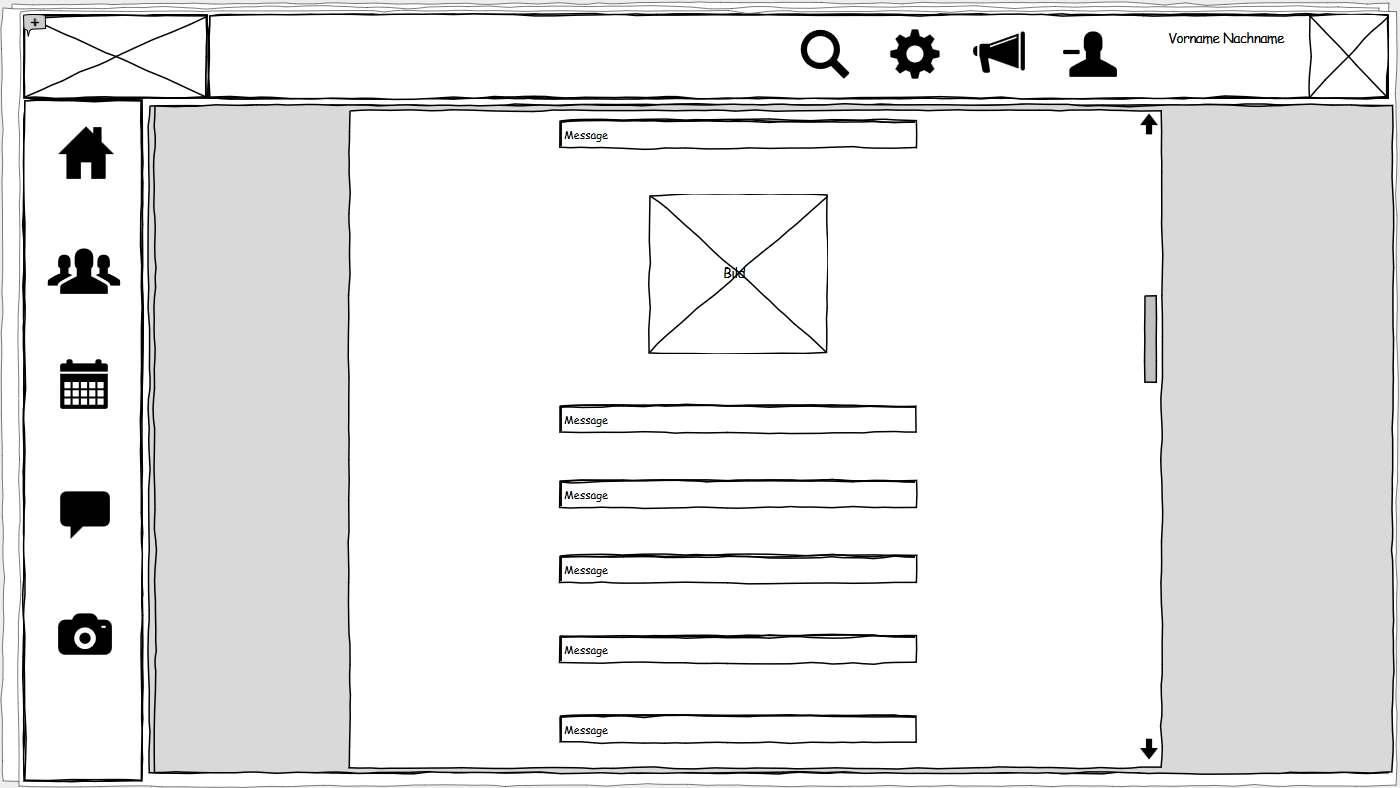
\includegraphics[width = 150mm]{pictures/Messageboard.PNG}
 \end{figure}
 
  \subsection{Templateseite Auditlog}
 \begin{figure}[ht!]
  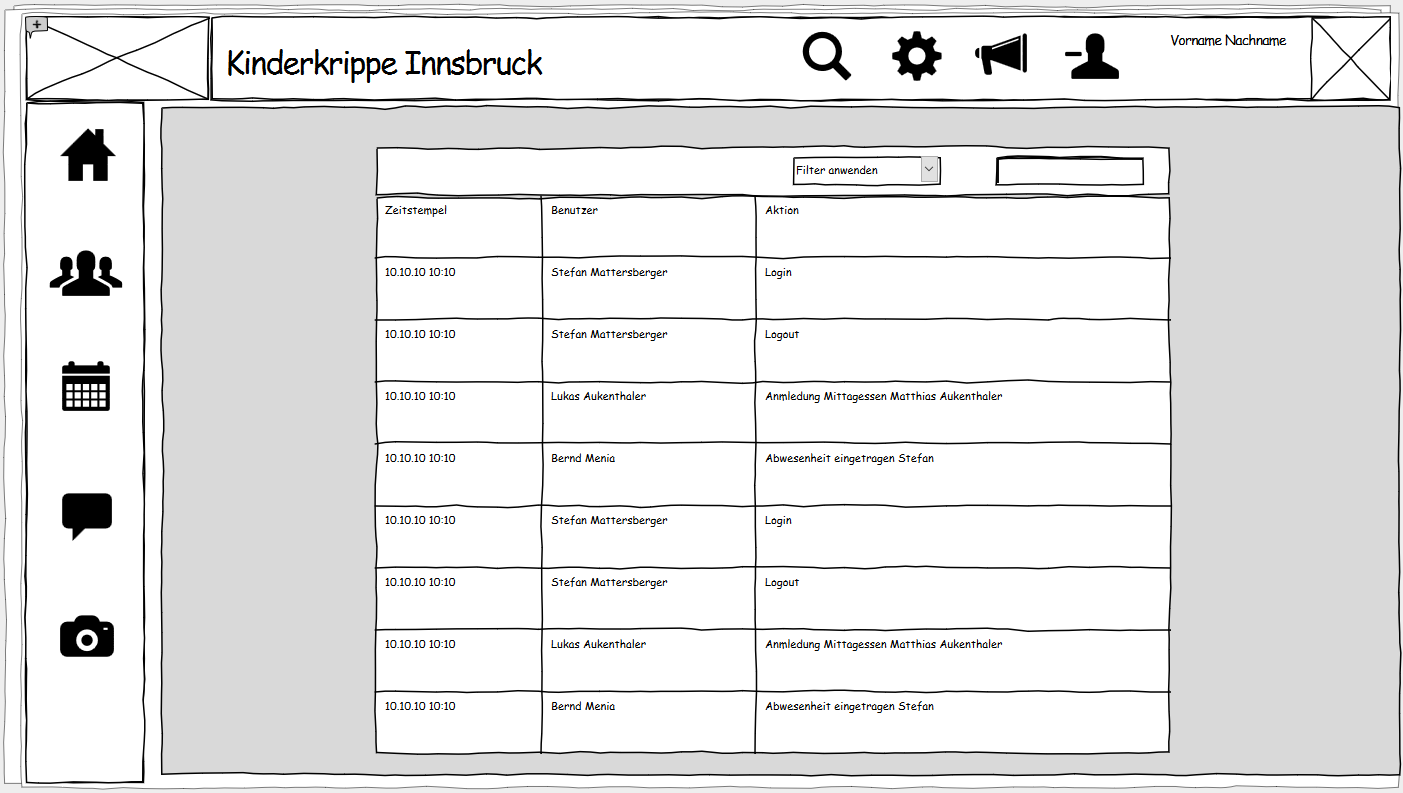
\includegraphics[width = 150mm]{pictures/Auditlog.PNG}
 \end{figure}
 
  \newpage
 \subsection{Templateseite Bildergalerie}
 \begin{figure}[ht!]
  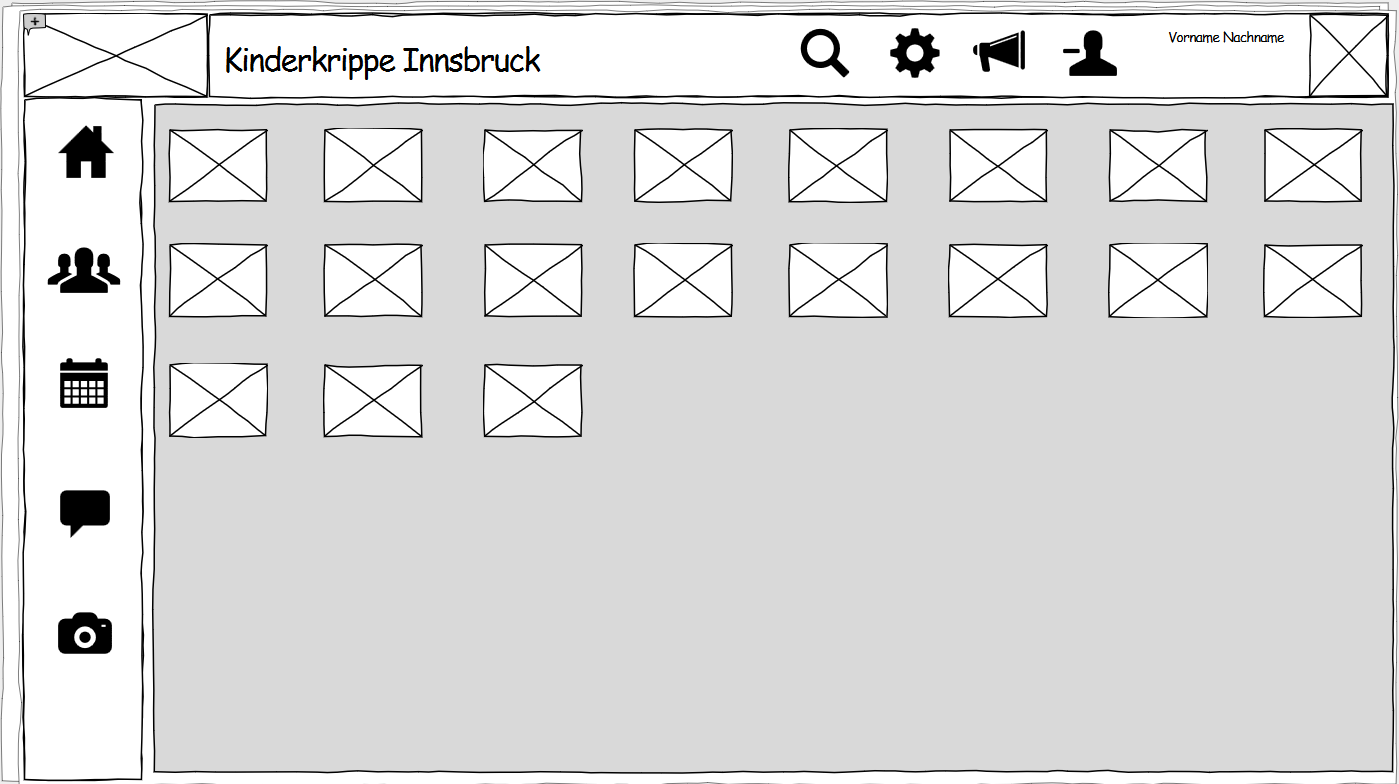
\includegraphics[width = 150mm]{pictures/Bildergalerie.PNG}
 \end{figure}
 
  \subsection{Templateseite Bildergalerie Detail}
 \begin{figure}[ht!]
  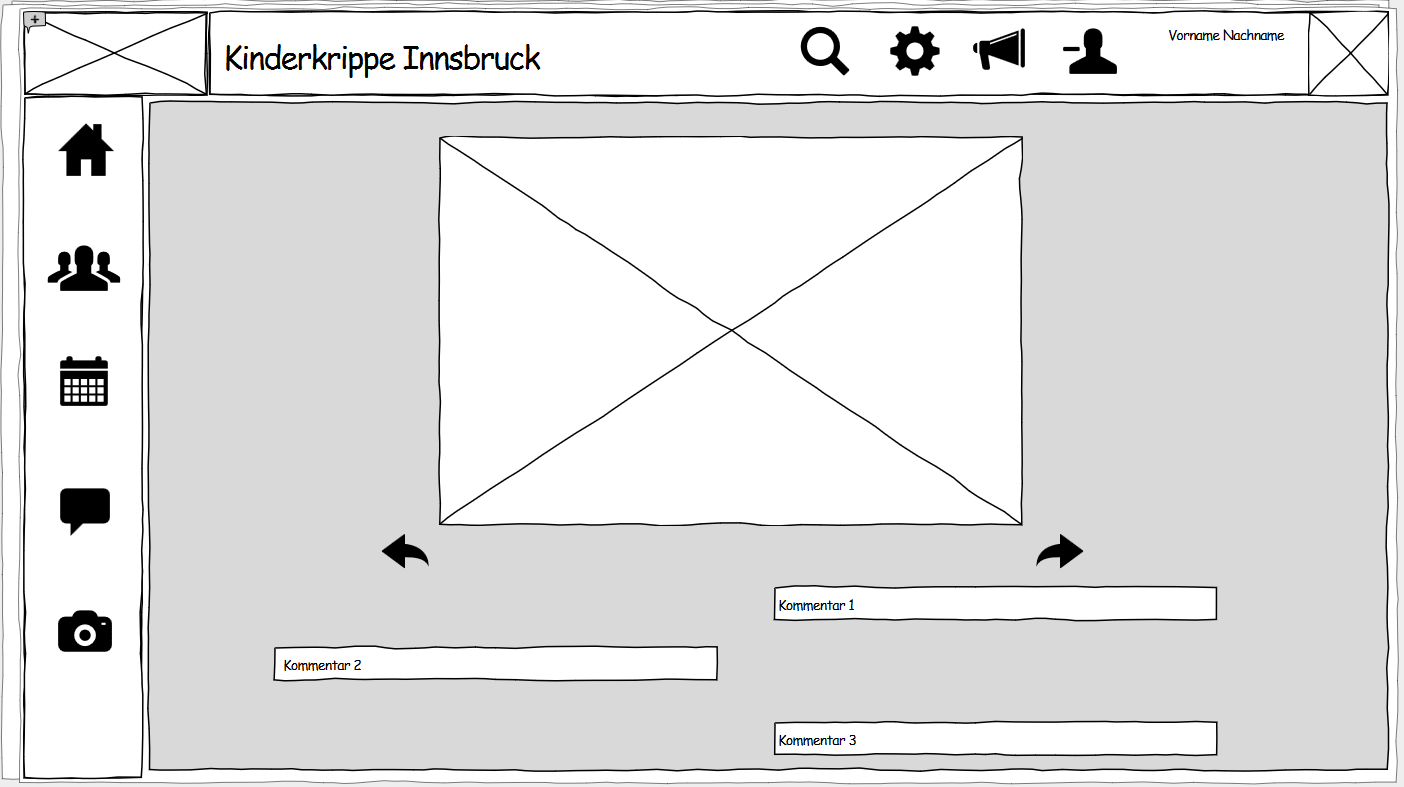
\includegraphics[width = 150mm]{pictures/Bildergalerie_detail.PNG}
 \end{figure}
 
